% !TEX TS-program = pdflatexmk
% Dissertation write up - 1967423

\documentclass[11pt]{article}

% Packages
\usepackage[margin = 1in, includefoot]{geometry}
\usepackage{setspace}
\usepackage{helvet}
\usepackage{natbib}
\usepackage{graphicx}

% Bib style
\bibliographystyle{agsm}

% Global commands
\renewcommand{\familydefault}{\sfdefault} % Set font as Helvetica (close enough to Arial)
\onehalfspacing % 1.5 line spacing

% Cover page details
\title{Trends in the pervasiveness of Central Bank conspiracy theories and its consequences for monetary policy: Mining ``Bank of England'' Twitter}
\author{Course code: IB9L1L\\
	    Candidate: 1967423\\
	    Wordcount: xxxx\footnote{According to TexCount Version 3.1, available at: \texttt{http://app.uio.no/ifi/texcount/}}}
\date{\today}

\begin{document}

\begin{titlepage}
	\centering
	\maketitle
\abstract{blah blah blah blah blah blah blah blah blah blah blah blah blah blah blah blah blah blah blah blah blah blah blah blah blah blah blah blah blah blah blah blah blah blah blah blah blah blah blah blah blah blah blah blah blah blah blah blah blah blah blah blah blah blah blah blah blah blah blah blah blah blah blah blah blah blah blah blah blah blah blah blah blah blah blah blah blah blah blah blah blah blah blah blah blah blah blah blah blah blah blah blah blah blah blah blah blah blah blah} 

\vspace{1in}

This is to certify that the work I am submitting is my own. All external references and sources are clearly acknowledged and identified within the contents. I am aware of the University of Warwick regulation concerning plagiarism and collusion.
No substantial part(s) of the work submitted here has also been submitted by me in other assessments for accredited courses of study, and I acknowledge that if this has been done an appropriate reduction in the mark I might otherwise have received will be made.
	
	\end{titlepage}
	
\section{Introduction} \label{Section: Introduction}

\section{Central Banks, Populism, and Conspiracy Theories} \label{Section: Central Banks, Populism, and Conspiracy Theories}

\subsection{Populism and central banks} \label{subsection: Populism and central banks}

The recent proliferation of populism has caused the concept to be among the hottest, and yet most controversial, topics in political science \citep{brubaker2020populism}. There is a lack of consensus on its definition, key characteristics, empirical extensions and even whether it represents a positive, negative or neutral political force \citep{bergmann2020populism, brubaker2020populism, caiani2019understanding}. The importance of populism is emphasised by authors suggesting it constitutes the second dimension to the left-right political spectrum \citep{koch2021varieties}. Some go so far as to say it has replaced the historic left-right cleavage \citep{de2018populism}. With reference to central banks, it is clear that populism transcends the left-right divide and populist rhetoric is found on both sides of the political spectrum. For example, the right-wing nationalist ex-president Donald Trump has referred to central bankers at the Federal Reserve as ``boneheads'' and urged them to keep interest rates low. His rhetoric is clearly nationalist and anti-elite in nature, stating on Twitter that ``it is incredible that with a very strong dollar and virtually no inflation, the outside world blowing up around us, Paris is burning and China way down, the Fed is even considering yet another interest rate hike. Take the Victory!'' \cite[pg.~9]{binder2021technopopulism}. On the other hand, left-wing presidential candidate Bernie Sanders has also engaged in populist discourse targeted towards the Federal Reserve. In an article from 2015, he suggested members of the Federal Reserve's boards should be reorganised to include ``representatives from all walks of life — including labor, consumers, homeowners, urban residents, farmers and small businesses'' \citep{sanders2015bernie}. What these two examples have in common is a general distrust for elites and a belief that the economic incumbents do not represent the best of interest of a homogenous `people'.

Why are central banks a target for populist rhetoric? As highlighted by the ex-Governor of the Reserve Bank of India, Raghuram Rajan, ``with their PhDs, exclusive jargon, and secretive meetings in far-flung places like Basel and Jackson Hole, central bankers are the quintessential rootless global elite that populist nationalists love to hate'' \citep{rajan2017central}. Central bankers represent the global elite that populists believe are disconnected with the needs of the people. Additionaly, populism is often interpreted as a direct response to the crisis of representation found in liberal representative democracies \citep{de2018populism}. There has been a gradual collapse in the legitimacy of mass parties' claims to broaden and represent their electoral base.  As \cite{de2018populism} explain, the cleavage between the people and their representatives has widened. The resulting void has been filled with a new approach to representation: bottom-up participation and direct democracy; the legitimation of authoritarian leaders who are the supreme representative for the people's interests; and the delineation between the people and the ``non-people'' composed of the elites. It is no surprise then, that central banks, who were gifted independence from direct political interference by the very parties who are now experiencing a crisis of legitimacy, are under fire from populists who are proponents of direct democracy and the will of the people. 

Furthermore, it is argued that the recent growth of populism has in part been cause by structural changes in the real economy and emphasised by the global financial crisis. \citep{gnan2020populism} highlight several economic factors including: (a) technological change leaving less educated, older and rural groups unable to adjust; (b) economic liberalisation, migration and labour market reforms attacking incumbents’ rents and wages; (c) globalisation raising fears of competition from low-cost countries; and (d) the rise of income and wealth inequality. Regulatory failings leading up to the financial crisis \citep{turner12017did} undermined the legitimacy of policy makers, regulators and central banks alike. As a key economic and regulatory institution, central banks are a symbol of the economic dissatisfaction that is fuelling populist movements across the globe.

In summary, central banks are (a) globalist institutions promoting technical expertise; (b) making decisions with limited direct democratic accountability and whose accountability via politicians that have lost legitimacy themselves; and (c) symbols of structural economic changes and the global financial crisis. These three factors mean it is no surprise that independent central banks find themselves in the firing line from populist leaders worldwide.

\subsection{From populism to conspiracy} \label{subsection: From populism to conspiracy}

Unlike the literature on populist rhetoric towards central banks, there is very little published work on central bank conspiracy theories. \cite{james2010central} suggests that central bank conspiracy theories are not a new phenomena in the United Kingdom. The author highlights a conspiratorial atmosphere in the aftermath of the great depression, including theories ``that central bank independence and international central bank cooperation were conspiracies to divert money away from a national community''  and that ``the Bank of England [orchestrated] a “Banker’s Ramp” which had used financial blackmail to force the government to cut unemployment benefits'' \citep[pg.~12]{james2010central}. \cite{tokle2005fed} studied several conspiracy theories in the context of economic education. These theories, published in Sheldon Emry's \textit{Billions for the Bankers, Debts for the People}, focussed on alternative interpretations of the history of the Federal Reserve, alleged market manipulation and misinformation about inflation. The author takes time to debunk these theories and explains how the process of correcting these conspiracy theories could be a useful tool for student learning about central banks and monetary policy. Finally, there is some work on the proliferation of antisemitic central bank conspiracy theories \citep[for example]{league2017jewish}.

Recent work has begun to explore the relationship between populism and conspiracy theories more generally. Authors in the past have demonstrated the relationship between extreme political views and conspiracy theories \citep{van2015political}. This implies, if we observe a general increase in political polarisation and extremism, we may see growing conspiratorial tendencies in the population. As we discussed above, populism isn't a dimension that is only associated with the extreme left or right, and hence the relationship between populism and conspiracy theories should be taken separately. \cite{castanho2017elite} studied the relationship between populist attitudes and conspiratorial beliefs. The authors first note similarities in the world-views of populists and conspiracy theorists. As outlined in Section \ref{subsection: Populism and central banks}, populists tend to see the world divided between a homogeneous malevolent elite and a homogenous people whose views are not considered by the elite. This is a view also shared by conspiracy theorists. Conspiracy theorists ``see conspirators controlling society, with more resources and willpower, and ordinary people as their victims'' \citep[pg.~427]{castanho2017elite}. The authors model the relationship between populist views and conspiratorial tendencies using data from two online surveys. They find holding a more populist view is correlated with some aspects of conspiracy theory belief. Specifically, populists are more likely to believe in conspiracies where a small group of powerful elites control world events and the dissemination of information for private gains at the expense of the people. They find no positive associated between populism and beliefs in acts of domestic terrorism by governments against there own citizens or the secretive and deliberate mass harm to the health and personal well-being of individuals. For our application and based on our exploration in Section \ref{subsection: Populism and central banks}, the first conspiratorial view seems the most relevant to central banks. However, there is no claim that this association is causal. It could be the case that conspiratorial individuals are more likely to be attracted to populist rhetoric, or that populist views naturally lead to conspiratorial tendencies in extremis. \cite{van2018populism} also outline the similarities in populism and conspiratorial tendencies along the themes of anti-elitism, anti-pluralism and threatened nationalism. Once again the authors indicate that conspiracy theories may be an intrinsic aspect of populism but cannot assign a causal mechanism.

One way populism could lead to conspiratorial tendencies is through the adoption of conspiracies by mainstream populist leaders and media. \cite{bergmann2020conspiracy} discuss how conspiracy theories merge with populist ideology and how populist leaders employ them to achieve their goals. The authors provide two case studies: Donald Trump perpetrating conspiracies in the lead up to the 2016 US presidential election and anti-immigrant conspiracy theories in the Nordic countries. \cite{sawyerpopulism} argues that conspiratorial narratives are employed by populist leaders to mobilise their base. This is achieved through two mechanisms: (1) as a method for the populist to demonise and delegitimise opponents, making it the imperative of voters to defeat them;  and (2) the populist can rally supporters by positioning themselves as a ``defender of the people'' who will restore order and decency to the country from the conspiring forces. It is easy to see how these methods are employed in the context of the US presidential election. A similar process has also been observed during the pandemic, where populist views may encourage conspiratorial views related to COVID-19 in part through conservative media \citep{stecula2021populism, eberl2021populism}.

This section has outlined a gap in central bank literature on the prevalence of conspiracy theories; set out previous evidence on the association between populism and conspiracy theories; and suggested one mechanism populism could lead to conspiracy is through the propagation of conspiracy theories by populist leaders and media. This is all to say, given recent increases in populist views of central banks we should see a similar (but delayed) increase in conspiracy narratives.

\subsection{Twitter analysis of conspiracy theories} \label{subsection: Twitter analysis of conspiracy theories}

This study takes place in the context of Twitter.  When studying the spread of conspiracy theories, social networks have been demonstrated to be a key amplifier \cite{kauk2021understanding}. \cite{cinelli2020covid} used epidemiological models to calculate the basic reproduction number, $R_0$, for information in several social media platforms. They found that the $R_0$ was supercritical in all of them. Twitter's reproduction rate was above that of Gab, Reddit and Youtube, but below the imagine-based Instagram. The spread of misinformation can be so extreme that \cite{bovet2019influence} argue that 25\% of news tweets relating to the 2016 US presidential election contained fake or highly biased information. The pervasiveness of misinformation can also be attributed to echo chambers \citep{cinelli2021echo} emerging on Twitter and other social media networks. Echo chambers are where social media limits exposure to differing perspectives and favours the formation of groups of like-minded users reinforcing a shared narrative. These factors make Twitter an interesting place to study the spread of conspiracy theories.

There is a huge number of studies that examine conspiracy narratives on Twitter, most recently relating to the COVID-19 pandemic \citep[to name a few]{eberl2021populism, jamison2020not, stephens2020geospatial}. \cite{jackson2021qanon} studied the proliferation of the modern QAnon conspiracy theory on Twitter. They extracted Tweets from the Twitter API that contained key words related to the QAnon conspiracy theory and filtered these based on several other rules to remove false positives. The authors studied the prevalence of QAnon-related tweets over time; the accounts taking part in the conspiracy; and key linguistic characteristics (such as common unigrams and bigrams). Another conspiracy covered by the analysis of Twitter data is 5G-COVID-19 misinformation \citep{ahmed2020covid, schroeder2021wico}. \cite{ahmed2020covid} studed 6,556 Twitter users whose tweets contained the ``5Gcoronavirus'' keyword or the \#5GCoronavirus hashtag through social network graph clusters. Another way of identifying conspiratorial tweets was undertaken by \cite{mahl2021nasa}, who searched for ten conspiracy theories using hashtag co-occurances. As explained in the paper, one limitation of this approach is that not all tweets contain a hashtag. This could lead to underrepresentation of conspiratorial views or sampling bias.

Studying conspiracy theories on Twitter is a deep and diverse field. Most studies choose their conspiracy theory before identifying the tweets, hence reduce the difficulty of their identification problem. Conspiratorial tweets are identified using key-word searches, identifying conspiracy touting users, or by searching for a list of hashtags (generated directly or by co-occurances). This article will add to the literature by proposing a method for studying overall conspiratorial sentiment related to a specific institution, concept or individual on Twitter. Previous studies take their identified corpus of tweets and perform analyses ranging from descriptive statistics on frequency, users and n-grams to more complex methods such as network analyses and clustering.

The next section will outline this paper's approach to identification and analysis.

\section{Studying ``Bank of England'' Twitter} \label{Section: Studying ``Bank of England'' Twitter}

\subsection{Methodological Approach} \label{Subsection: Methodological Approach}

The key methodological challenge for this paper is quantifying the \textit{amount} of conspiracy rhetoric in a set of Tweets. This paper will employ two methods and compare their results. The first will be a categorical approach where a given Tweet is given a binary classification of `conspiratorial' or `not conspiratorial' based on the occurrence of words from a fixed conspiracy-dictionary. This is similar to the approach employed by previous work referenced above \citep{jackson2021qanon, ahmed2020covid}. However, there are several limitation to dictionary-based approaches, such as the misclassification of terms that have meanings outside of conspiratorial circles and linguistic ambiguity, which we explain in more depth later. Our second approach will consider how similar tweets are to some ground-truth conspiratorial source. This approach will place the tweets on a continuous scale meaning that the definition of when a tweet is conspiratorial is arbitrary. The benefit of this approach is that we can model characteristics of the texts which would be missed by a dictionary led approach. However, a lot of these approach face challenges of sample size with the small word-count tweets.

\subsection{Data collection and summary} \label{Subsection: Data collection and summary}
\subsection{Topic Modelling} \label{Subsection: Topic Modelling}

Another way we can describe our dataset is through the types of topics that are under discussion. To break the tweets into categories we employ a Biterm Topic Model (BTM). Introduced by \cite{yan2013biterm}, the BTM builds upon earlier topic models such as the Latent Dirichlet Allocation (LDA) \citep{blei2003latent} and correlated topic models (CTMs) \citep{blei2006correlated}. These early topic models rely implicitly on word co-occurances within documents to generate their topics. For a dataset (or `corpus' in natural language processing) with a large number of short texts, this can lead to huge data sparsity. That is, a very large dictionary of words where very few words appear in each text; a large document-term matrix where most entries are 0. The BTM attempts to solve this problem by directly modelling the generation of word co-occurrences (i.e. biterms) in the whole corpus rather than within individual documents. A biterm is an unordered word-pair co-occurring within a text. For example, the sentence ``we model biterms'' has 3 biterms: ``we-model``, ``model-biterms'', ``we-biterms''. Since they are unordered, ``we-model'' is the same as ''model-we''. Conceptually, the whole corpus is treated as a mixture of topics, where each biterm is drawn independently from a specific topic. The probability that a biterm drawn from a specific topic is further captured by the chances that both words in the biterm are drawn from the topic \citep{yan2013biterm}.

The BTM has repeatedly been shown to outperform traditional topic models for short texts \citep{yan2013biterm, jonsson2015evaluation, chen2015user}. As such, many authors have used the BTM on Twitter data for a variety of diverse applications \citep[to name a few]{mackey2018solution, han2016exploratory, khan2021twitter}. While the algorithm is unsupervised, the researcher is required to select the number of topics that the texts will be split into ($K$). There are a variety of approaches to help the researcher select the best $K$, but these should act as a guide and cannot replace a subjective visual analysis on the quality of the topics. One approach to help pin down potential $K$s is semantic coherence, introduced by \cite{mimno2011optimizing}. Semantic coherence is maximised when the most probable words in a topic frequently occur near one another in the original text and correlates particularly well with the human judgment of topic quality. For a given fitted topic model, a semantic coherence score is given to each topic, the result can be averaged to give a score for the model as a whole.

Before training the model, the corpus goes through a number of pre-processing steps to remove information which is not relevant to topic classification and may misdirect the unsupervised model. We convert the texts to lower case, remove punctuation, stem words and remove stopwords (e.g. a, he, she, they, to). Stemming is the process by which words are reduced to their root. This means words such as \emph{banking} and \emph{banker} are reduced to \emph{bank}, thereby aiding with their accurate clustering by explicitly telling the model they have similar semantic meanings. The final pre-processing step is removing the reference to the Bank of England - ``bank of england''\footnote{In reality, this is done before removing stopwords because ``of'' is a stopword.}, ``boe'' or ``bankofengland''. The way we collected our sample means these words are present in every tweet. Therefore, they constitute the most probable word for each topic and the best fit for $K$ is less than five. Subjectively, it would seem the true number of topics relating to the Bank of England over ten years is more than five. Evidence for this phenomena is available in Appendix A. 

\begin{figure}[h]
	\center
	\caption{Semantic coherence for BTM models with varying $K$} \label{fig:k search}
	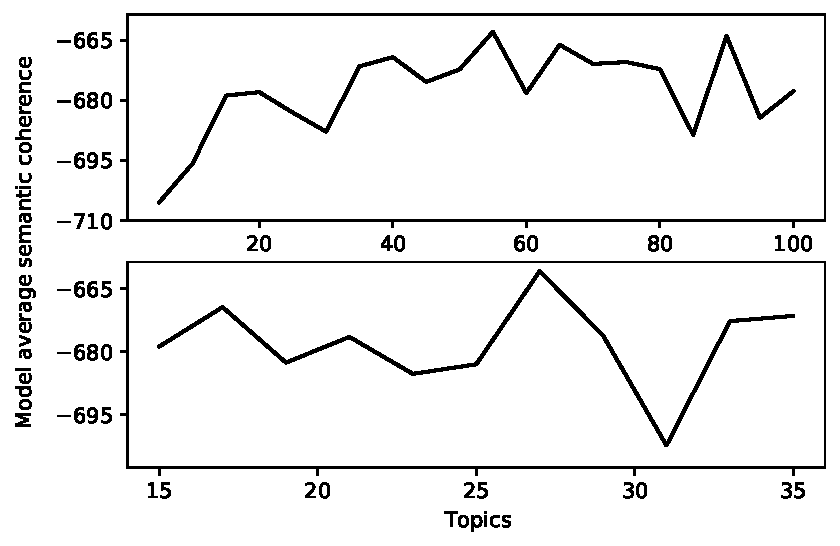
\includegraphics[keepaspectratio = true]{k_search.pdf}
	\end{figure}

The top panel of Figure \ref{fig:k search} gives model average semantic coherence for BTMs with between five and 100 topics in steps of five. Forgoing the noise, we can see that semantic coherence first rises sharply, before the rate of change falls, and little additional coherence is gained from going beyond 35 topics. For our purposes, we have to evaluate the trade-off between improved average topic coherence and more difficult interpretation. The labelling of topics is done manually, so a large number of topics means assigning meaning becomes more costly and simpler interpretation becomes more difficult. Therefore, we tend to want to find a range of $K$ that minimises the number of topics for an acceptable coherence level. The bottom panel of Figure \ref{fig:k search} drills down into $K$s between 15 and 35 in steps of two. Given coherence changes very little within this range, I ran estimations at between 15 and 20 topics and evaluated the outputs manually.


\subsection{Dictionary-based classification} \label{Subsection: Dictionary-based classification}
\subsection{Similarity index} \label{Subsection: Similarity index}

\section{Discussion} \label{Section: Discussion}

\clearpage
\bibliography{IB9L1L_bib.bib}

\end{document}